
Luego de haber explicado las debilidades del protocolo \emph{HTTP}, vamos a explorar las 
distintas soluciones encontradas, empezando con un pequeño marco teórico, el cual 
nos permitirá probar estas implementaciones y aplicarlas en un escenario de prueba.

La herramienta utilizada es \emph{Docker}, con ella es posible simular 
escenarios sin necesidad de tener cada uno de los servidores de manera física. Para
entenderlo un poco mejor, explicaremos lo que es la virtualización y profundizaremos 
en la virtualización basada en contenedores.
    
\section{Máquinas virtuales}

La virtualización brinda la capacidad de ejecutar aplicaciones, sistemas 
operativos o servicios del sistema en un entorno distinto. 
Obviamente, los mismos tienen que estar ejecutándose en un determinado 
sistema informático en un momento dado, pero la virtualización proporciona 
un nivel de abstracción lógica que libera las aplicaciones, los servicios 
del sistema e incluso el sistema operativo de estar vinculado a una 
pieza específica de \emph{hardware}. El enfoque de la virtualización hace 
que todo esto sea portátil a través de diferentes sistemas informáticos 
físicos.

El enfoque basado en \emph{VM} virtualiza el sistema operativo completo. Con esto nos referimos 
a la virtualización de discos, \emph{CPU} y \emph{NIC}. En otras palabras, podemos afirmar que se 
trata de virtualizar la arquitectura de conjunto de instrucciones completa, como ejemplo, 
la arquitectura \emph{x86}. 

\begin{center}
    \begin{figure}   
       \begin{center}
          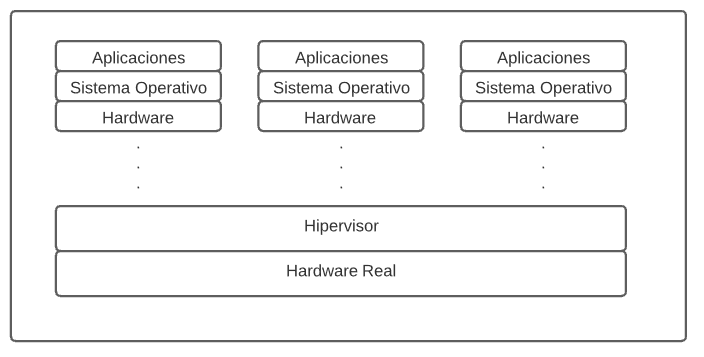
\includegraphics[width=12cm,height=7cm]{vm.png}
       \end{center}
       \caption{Virtualización}
    \end{figure}
 \end{center}

Para virtualizar un sistema operativo, se utiliza un \emph{software} especial, denominado
\emph{hipervisor}, y es el encargado, entre otras cosas, de aislar el sistema 
operativo de las máquinas virtuales y 
permitir crearlas y gestionarlas.

Una \emph{VM} debe satisfacer tres propiedades:
\begin{itemize}
    \setlength\itemsep{-0.6em}
    \item Aislamiento: debe aislar a los invitados entre sí. 
    \item Equivalencia: debe comportarse igual, con o sin virtualización. Esto 
    significa que se deben ejecutar la mayoría de las instrucciones en el \emph{hardware} 
    físico sin ninguna traducción hacia el \emph{hardware} virtual.
    \item Rendimiento: Debería funcionar tan bien como lo hace sin ninguna 
    virtualización. Esto nuevamente significa que la sobrecarga de ejecutar 
    una VM debe ser mínima.
\end{itemize}

\section{Virtualización basada en Contenedores}

Esta forma de virtualización no abstrae el \emph{hardware}, sino que utiliza técnicas 
dentro del \emph{kernel} de Linux para aislar las rutas de acceso para diferentes recursos. 
Establece un límite lógico dentro del mismo sistema operativo. Como resultado, obtenemos 
un sistema de archivos raíz separado, un árbol de procesos separado, un subsistema 
de red separado, etc.

\begin{center}
    \begin{figure}   
       \begin{center}
          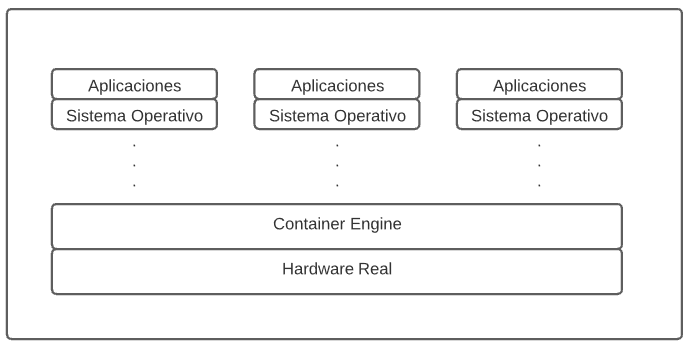
\includegraphics[width=12cm,height=7cm]{contenedores.png}
       \end{center}
       \caption{Virtualización basada en Contenedores}
    \end{figure}
 \end{center}

El \emph{kernel} de Linux se compone de varios componentes y funcionalidades; los relacionados 
con contenedores son los siguientes:
\begin{itemize}
    \setlength\itemsep{-0.6em}
    \item Grupos de control (\emph{Cgroups})
    \item Espacios de nombres (Namespaces)
    \item Linux con seguridad mejorada (SELinux)
\end{itemize}

\subsection*{Cgroups}
La funcionalidad de \emph{cgroup} permite limitar y priorizar recursos, como \emph{CPU}, RAM, 
la red, el sistema de archivos, etc. El objetivo principal es no exceder los 
recursos, para evitar desperdiciar recursos que podrían ser necesarios para 
otros procesos.

\subsection*{Espacios de nombres}
La funcionalidad del espacio de nombres permite particionar los recursos del kernel, 
de modo que un conjunto de procesos ve un conjunto de recursos, mientras que otro 
conjunto de procesos ve un conjunto diferente de recursos. La característica funciona 
al tener el mismo espacio de nombres para estos recursos en los distintos conjuntos 
de procesos, pero esos nombres se refieren a recursos distintos. Algunos nombres 
de recursos que pueden existir en varios espacios son los ID de proceso, nombres 
de host, ID de usuario, nombres de archivo y algunos nombres asociados con el 
acceso a la red y la comunicación entre procesos. 

Cuando se inicia un sistema 
Linux, solo se crea un espacio de nombres. Los procesos y recursos se unirán 
al mismo espacio de nombres, hasta que se cree un espacio de nombres diferente, 
se le asignen recursos y los procesos se unan a él.

\subsection*{SELinux}
SELinux es un módulo del \emph{kernel} de Linux que proporciona un mecanismo para hacer 
cumplir la seguridad del sistema, con políticas específicas. Básicamente, SELinux 
puede limitar el acceso de los programas a archivos y recursos de red. La idea es 
limitar los privilegios de los programas y demonios al mínimo, de modo que pueda 
limitar el riesgo de que el sistema se detenga.

Lo contenedores utilizan los recursos directamente y no necesitan de un emulador en 
absoluto, cuantos menos recursos, mayor eficiencia. Se pueden ejecutar diferentes 
aplicaciones en el mismo host: aisladas a nivel de \emph{kernel} y aisladas por 
espacios de nombres y \emph{cgroups}. El \emph{kernel}, es decir, el Sistema Operativo,
 lo comparten todos los contenedores.

\subsection*{Contenedores}
Cuando hablamos de contenedores, nos referimos indirectamente a dos conceptos 
principales: una imagen de contenedor y una imagen de contenedor en ejecución. 
Una imagen de contenedor es la definición del contenedor, en donde el \emph{software} 
restante se instala como capas adicionales, como se muestra en el diagrama.

\begin{center}
    \begin{figure}   
       \begin{center}
          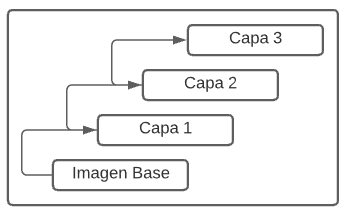
\includegraphics[width=7.5cm,height=5cm]{contenedores-capas.png}
       \end{center}
       \caption{Capas de contenedores}
       \label{capasContenedores}
    \end{figure}
 \end{center}

Una imagen de contenedor suele estar formada por varias capas (figura \ref{capasContenedores}).
La primera capa está dada por la imagen base, que proporciona las funcionalidades 
centrales del sistema operativo, con todas las herramientas necesarias para comenzar. 
Los equipos de desarrolladores a menudo trabajan construyendo sus propias capas sobre 
estas imágenes base. Los usuarios también pueden crear imágenes de aplicaciones más 
avanzadas, que no solo tienen un sistema operativo, sino que también incluyen 
herramientas de depuración y bibliotecas.

Los contenedores brindan aislamiento al aprovechar las tecnologías del \emph{kernel}, como 
\emph{cgroups}, espacios de nombres del \emph{kernel} y SELinux. Dado que  
utilizan un \emph{kernel} compartido y un host de contenedor, se reduce la cantidad de 
recursos necesarios para el contenedor en sí y son más livianos en comparación 
con las máquinas virtuales. 

Por lo mencionado anteriormente, podemos afirmar que los contenedores brindan una agilidad 
que no es factible con las \emph{VM}, y una prueba de esto es que solo se 
necesitan unos segundos para iniciar un nuevo contenedor. 
Además, los mismos admiten un 
modelo más flexible en lo que respecta a la utilización de la \emph{CPU} y los recursos 
de memoria, y permiten modos de ráfaga de recursos, donde las aplicaciones 
pueden consumir más recursos cuando es requerido, dentro de los límites definidos.


\section{\emph{Docker}}

\emph{Docker} es una herramienta de código abierto que automatiza la implementación de aplicaciones 
en contenedores. Fue escrito por el equipo de \emph{Docker} y publicado por ellos bajo la 
licencia Apache 2.0. Está diseñado para proporcionar 
un entorno ligero y rápido para implementar escenarios determinados, así como un flujo de 
trabajo 
eficiente para llevar ese código desde una computadora portátil a su entorno de prueba 
y luego a producción. De hecho, se puede comenzar con \emph{Docker} en un host mínimo que 
no ejecute nada más que un \emph{kernel} de Linux compatible y un binario de \emph{Docker}.



\subsection{Imágenes}
Las imágenes son los componentes básicos del mundo de \emph{Docker}. El uso común es 
lanzando los contenedores a partir de imágenes. Tienen un formato en capas, que 
se forman paso a paso utilizando una serie de instrucciones.

Se puede considerar a las imágenes como el “código fuente” de los contenedores. 
Son muy portátiles y se pueden compartir, almacenar y actualizar. .

\subsection{Registros}
\emph{Docker} almacena las imágenes que se crean en registros. Hay dos tipos de 
registros: públicos y privados. La herramienta opera el registro público de imágenes, 
llamado \emph{Docker} Hub. Se puede crear una cuenta y usarla para 
compartir y almacenar nuestras propias imágenes. También es posible almacenar 
las imágenes que desee y mantenerlas privadas en \emph{Docker} Hub. Estas imágenes 
pueden incluir código fuente u otra información de propiedad que se quiera 
mantener segura o solo compartir con otros miembros de su equipo u organización.

\subsection{Contenedores}
El \emph{software} permite construir e implementar contenedores dentro de los cuales se puede 
empaquetar aplicaciones y servicios. Como acabamos de mencionar, los contenedores 
se lanzan a partir de imágenes y estos pueden contener uno o más procesos en ejecución.

\noindent Un contenedor es:
\begin{itemize}
    \setlength\itemsep{-0.6em}
    \item Un formato de imagen.
    \item Un conjunto de operaciones estándar.
    \item Un entorno de ejecución.
\end{itemize}

Se puede hacer una analogía entre los contenedores de \emph{Docker} y los contenedores 
de envío estándar, utilizado para transportar mercancías a nivel mundial. 
En lugar de enviar mercancías, los contenedores de \emph{Docker} envían \emph{software}. 
Cada contenedor contiene una imagen de \emph{software}, su “carga”, y, al igual 
que su contraparte física, permite realizar un conjunto de operaciones. 
Por ejemplo, se puede crear, iniciar, detener, reiniciar y destruir. Como 
un contenedor de envío, \emph{Docker} no se preocupa por el contenido del contenedor 
cuando realiza estas acciones; por ejemplo, si un contenedor es un servidor \emph{web}, 
una base de datos o un servidor de aplicaciones. Cada contenedor se carga 
igual que cualquier otro. A \emph{Docker} tampoco le importa dónde envía su contenedor: 
se puede compilar en una computadora portátil, cargarlo en un registro, luego 
descargarlo en un servidor físico o virtual, probarlo, implementarlo en un 
clúster de una docena de \emph{hosts} y ejecutarlo. 


